\documentclass[crop=true,border=0.2cm]{standalone}
\usepackage{textcomp}
\usepackage{tikz}
\usetikzlibrary{positioning}

\definecolor{softorange}{HTML}{ff7f0e}
\definecolor{softgreen}{HTML}{2ca02c}
\definecolor{softblue}{HTML}{1f77b4}
\definecolor{softred}{HTML}{d62728}

% boe template seems to use a smaller document-wide font size
%\renewcommand{\normalsize}{\small}%
%\renewcommand{\scriptsize}{\tiny}%

\begin{document}%
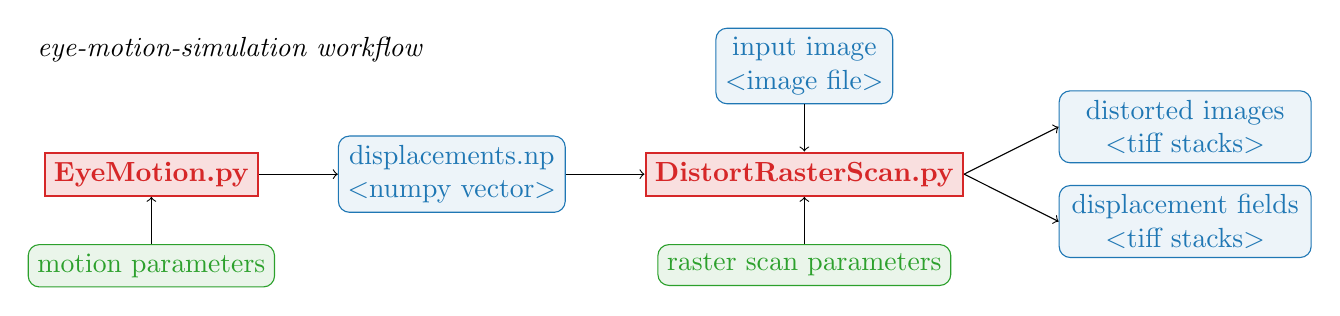
\begin{tikzpicture}[align=center,->]
	\tikzstyle{codefile}=[draw,rectangle,color=softred,fill=softred!15,thick,font=\bfseries]
	\tikzstyle{datafile}=[draw,rounded corners,color=softblue,fill=softblue!8]
	\tikzstyle{params}=[draw,rounded corners,color=softgreen,fill=softgreen!10]

	\node[codefile](eye_motion){EyeMotion.py};
	\node[params,below=0.6cm of eye_motion](motion_params){motion parameters};

	\node[datafile,right=of eye_motion](displacements){displacements.np\\$<$numpy vector$>$};

	\node[codefile,right=of displacements](distort_raster_scan){DistortRasterScan.py};
	\node[datafile,above=0.6cm of distort_raster_scan](input_image){input image\\$<$image file$>$};
	\node[params,below=0.6cm of distort_raster_scan](raster_scan_params){raster scan parameters};

	\node[datafile,above right=-0.15cm and 1.2cm of distort_raster_scan,minimum width=3.2cm](distorted_images){distorted images\\$<$tiff stacks$>$};
	\node[datafile,below right=-0.15cm and 1.2cm of distort_raster_scan,minimum width=3.2cm](displacement_fields){displacement fields\\$<$tiff stacks$>$};

	\node[anchor=north west] at (motion_params.west|-input_image.north){\textit{eye-motion-simulation workflow}};

	\draw(motion_params) -- (eye_motion);

	\draw(eye_motion) -- (displacements);

	\draw(displacements) -- (distort_raster_scan);
	\draw(input_image) -- (distort_raster_scan);
	\draw(raster_scan_params) -- (distort_raster_scan);

	\draw(distort_raster_scan.east) -- (distorted_images.west);
	\draw(distort_raster_scan.east) -- (displacement_fields.west);
\end{tikzpicture}%
\end{document}
